%*******************************************************
% Capitulo siete
%*******************************************************

\chapter{Capa de aplicación}

\marginpar{
    \begin{figure}[H]
        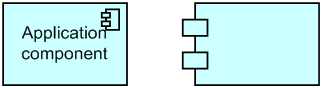
\includegraphics[scale=0.6]{IAplication_component}
    \end{figure} 
    \footnotesize 
    \textbf{Componente}.Una parte modular, desplegable, y reemplazable de un sistema de software que encapsula su comportamiento y los datos y expone estos a través de un conjunto de interfaces. 
\newline
}La capa de aplicación describe los componentes lógicos que integran la solución que sirve a los intereses de la organización. A continuación se describen los puntos de vista de la capa.

\section{Comportamiento de aplicación}
El punto de vista del comportamiento de aplicación describe el comportamiento interno de una solicitud; por ejemplo, como se da cuenta de uno o más servicios de aplicación. Este punto de vista es útil en el diseño del comportamiento principal de aplicaciones, o en la identificación de solapamiento funcional entre diferentes aplicaciones.

\begin{figure}[H]
\centering
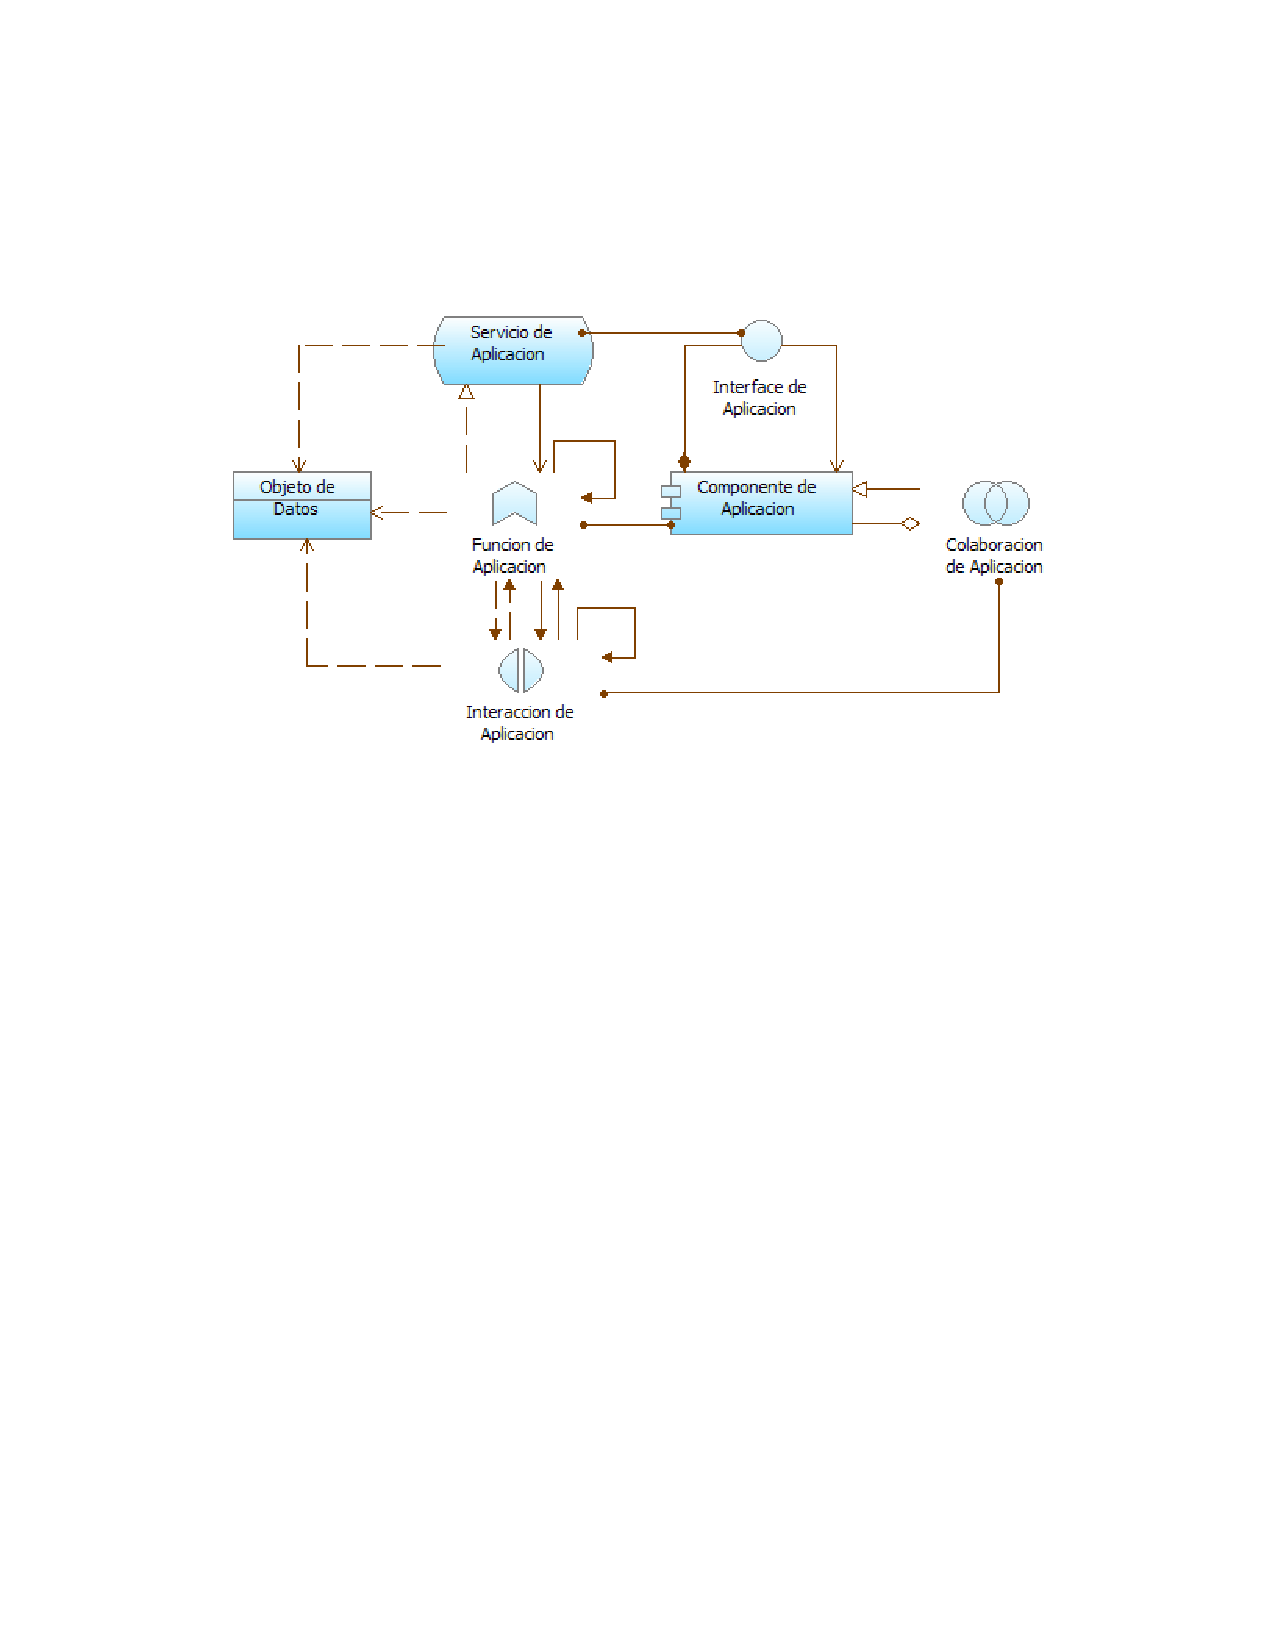
\includegraphics[scale=0.7]{comportamiento_de_aplicacion}
\caption{Metamodelo del punto de vista de comportamiento de aplicación.}
\end{figure}

\marginpar{
    \begin{figure}[H]
        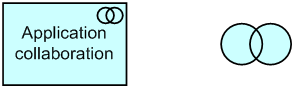
\includegraphics[scale=0.5]{IApplication_collaboration}
    \end{figure} 
    \footnotesize 
    \textbf{Colaboración}. Un agregado de dos o más componentes de aplicaciones que funcionan en conjunto para llevar a cabo un comportamiento colectivo.
\newline
}

Identificados los tres servicios principales, se describe una estructura de componentes que cumple las funciones de gestionar las calificaciones, comparar las marcas y gestionar comentarios específicos que complementan la calificación. Otros servicios no incluidos en el punto de vista pueden ser la gestión de la información de la marca por su dueño.

\begin{figure}[H]
\centering
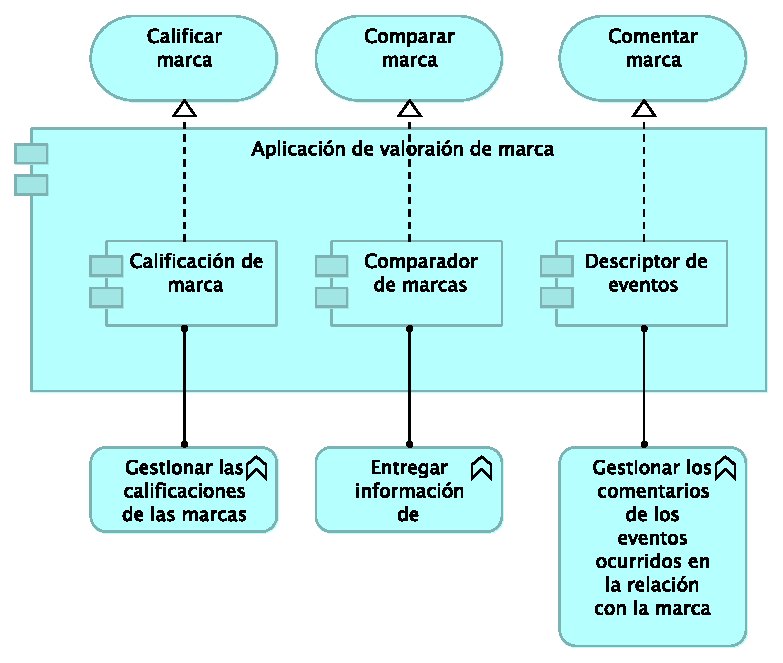
\includegraphics[scale=0.7]{Mcomportamientoaplicacion}
\caption{Punto de vista de comportamiento de aplicación.}
\end{figure}

\section{Cooperación de aplicación}
\marginpar{
    \begin{figure}[H]
        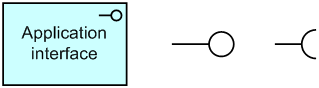
\includegraphics[scale=0.6]{IApplication_interface}
    \end{figure} 
    \footnotesize 
    \textbf{Interfaces}. Un punto de acceso donde se pone a disposición un servicio de aplicaciones para un usuario u otro componente de la aplicación
\newline
}El punto de vista de Cooperación de aplicación describe las relaciones entre los componentes de las aplicaciones en función de los flujos de información entre ellos, o en términos de los servicios que ofrecen y su uso. Es usado con frecuencia para crear una visión general del entorno de aplicaciones de una organización; también se utiliza para expresar la cooperación o la orquestación (interna) de los servicios que en conjunto apoyan la ejecución de un proceso de negocio.

\begin{figure}[H]
\centering
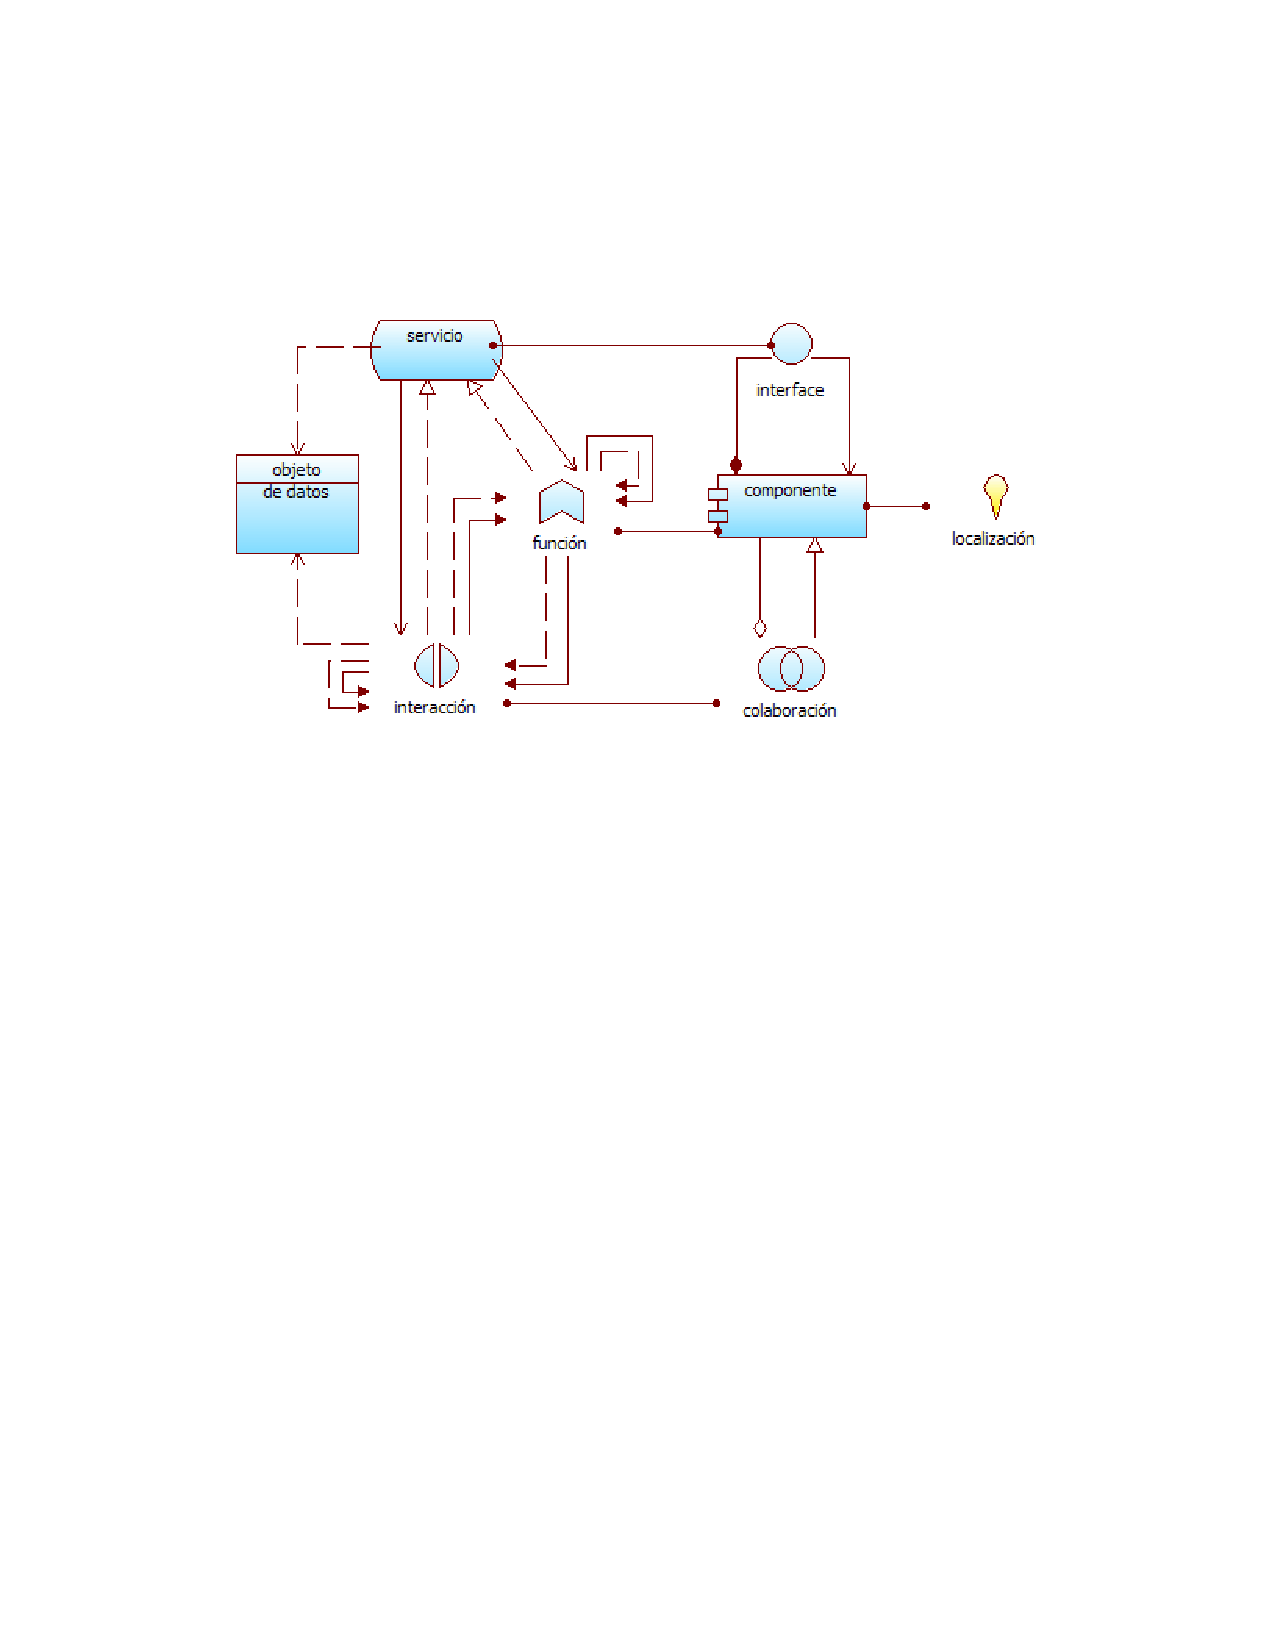
\includegraphics[scale=0.8]{cooperacion_de_aplicacion}
\caption{Metamodelo del punto de vista de Cooperación de aplicación.}
\end{figure}


\marginpar{
    \begin{figure}[H]
        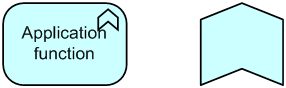
\includegraphics[scale=0.6]{IApplication_function}
    \end{figure} 
    \footnotesize 
    \textbf{Función}. Un elemento de comportamiento que grupos un comportamiento automático que puede ser realizado por un componente de aplicación.
}

En la cooperación de aplicaciones vale la pena destacar que las fuentes de datos para obtener información que permita valorar no solo provienen de las experiencias de usuario registradas en la aplicación sino también de la minería de datos desde redes sociales u otras aplicaciones.

\begin{figure}[H]
\centering
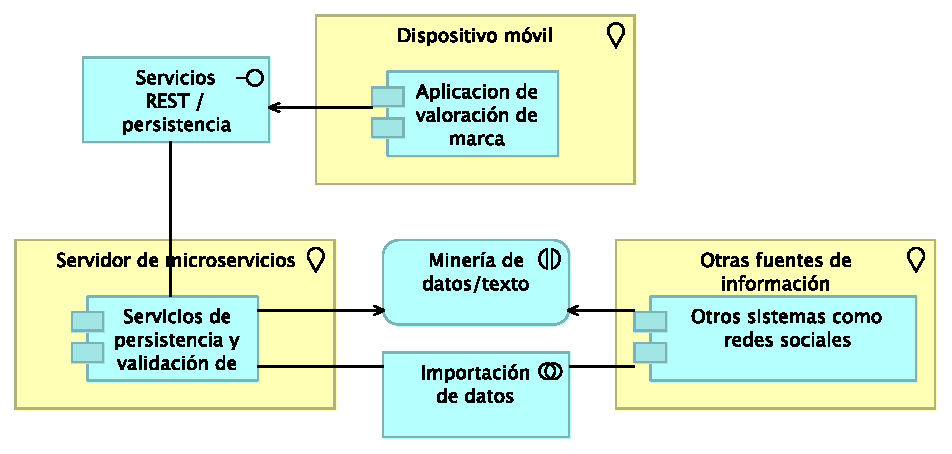
\includegraphics[scale=0.8]{Mcooperacionaplicacion}
\caption{Punto de vista de Cooperación de aplicación.}
\end{figure}


\section{Estructura de aplicación}
\marginpar{
    \begin{figure}[H]
        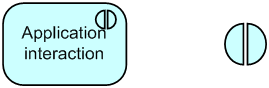
\includegraphics[scale=0.6]{IApplication_interaction}
    \end{figure} 
    \footnotesize 
    \textbf{Interacción}. es un elemento que describe el comportamiento de una colaboración de aplicación.
\newline
}El punto de vista estructura de la aplicación muestra la estructura de una o más aplicaciones o componentes. Este punto de vista es útil en el diseño o la comprensión de la estructura principal de aplicaciones o componentes y los datos asociados; por ejemplo, para romper la estructura del sistema en construcción, o para identificar los componentes de aplicaciones heredadas que son adecuados para la migración/integración.

\begin{figure}[H]
\centering
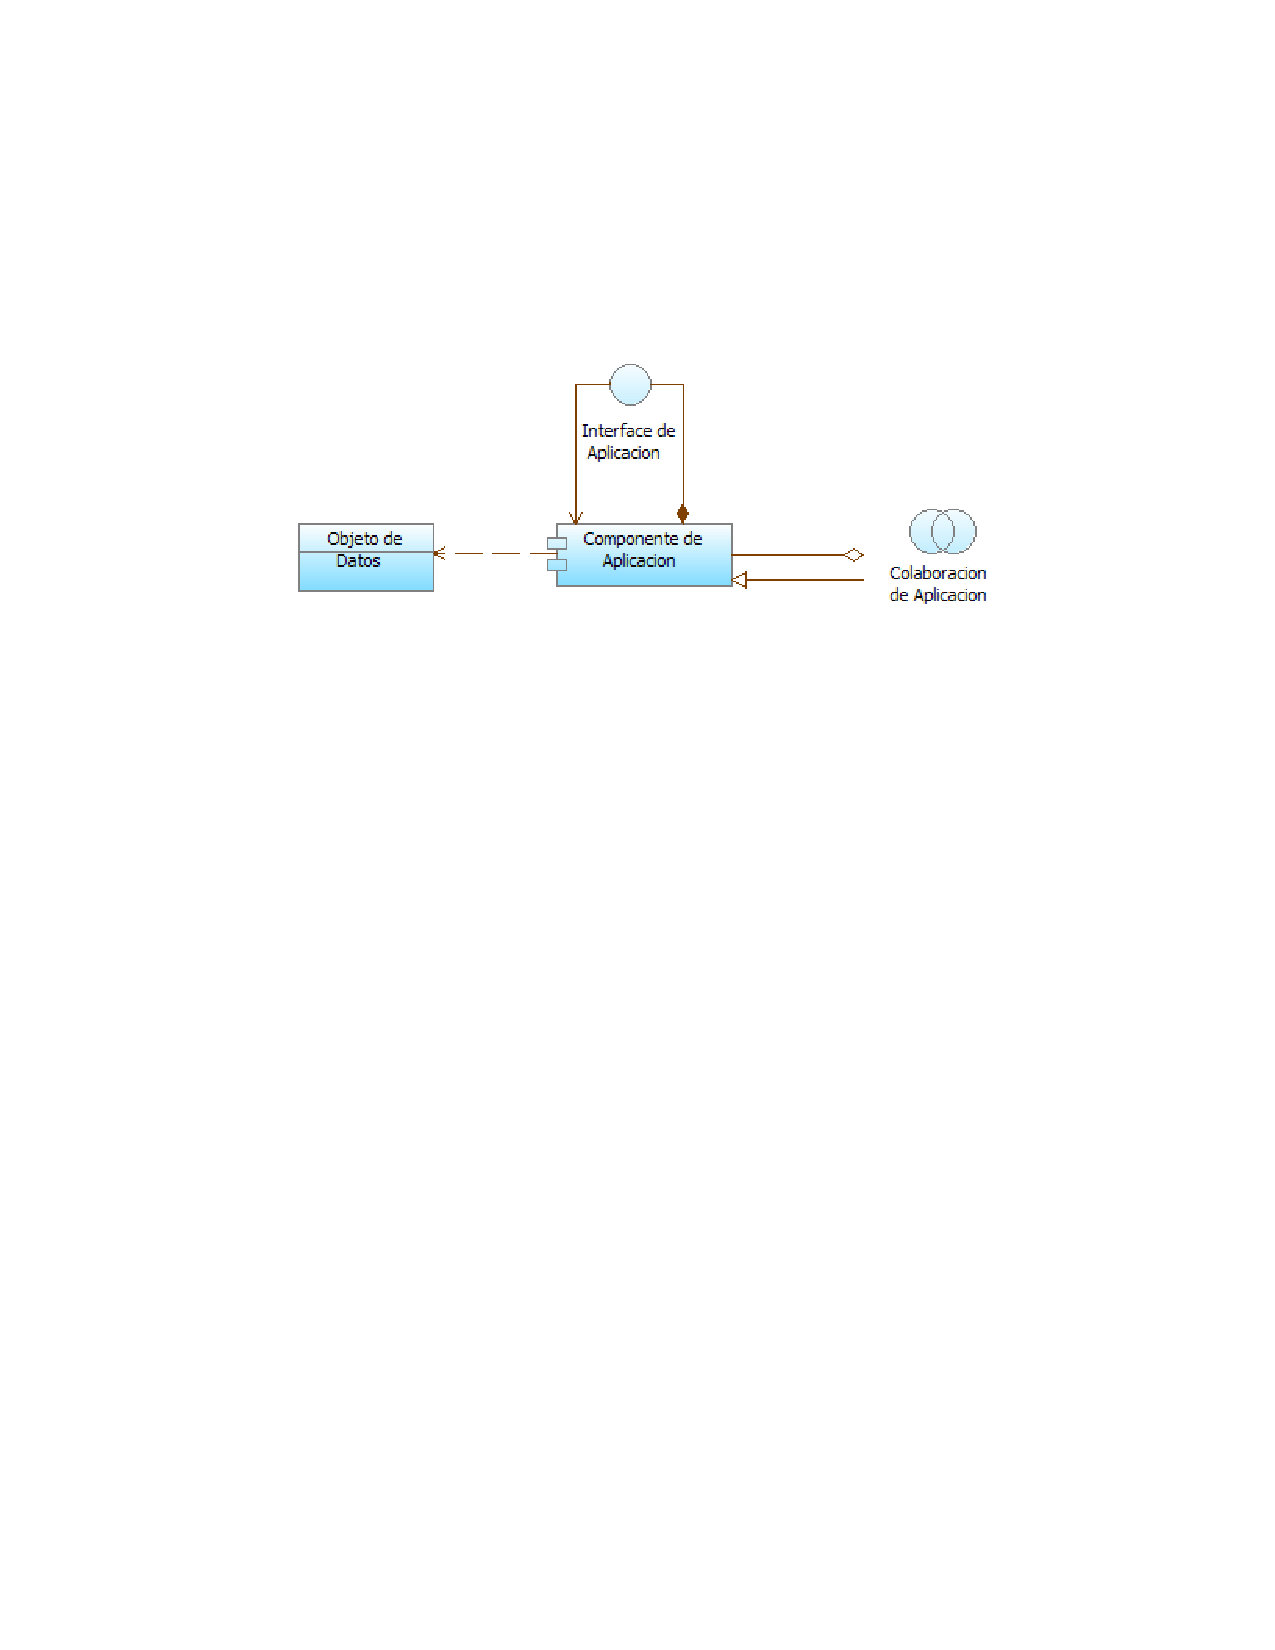
\includegraphics[scale=0.7]{estructura_de_aplicacion}
\caption{Metamodelo del punto de vista de Estructura de aplicación.}
\end{figure}

El modelo de componentes está descrito por la siguiente figura \ref{Mestructuraaplicacion}. Es de resaltar la propuesta de servicios REST expuestos desde el servidor de aplicaciones y consumo desde la aplicación móvil y desde una aplicación WEB de gestión de información de marca.

\begin{figure}[H]
\centering
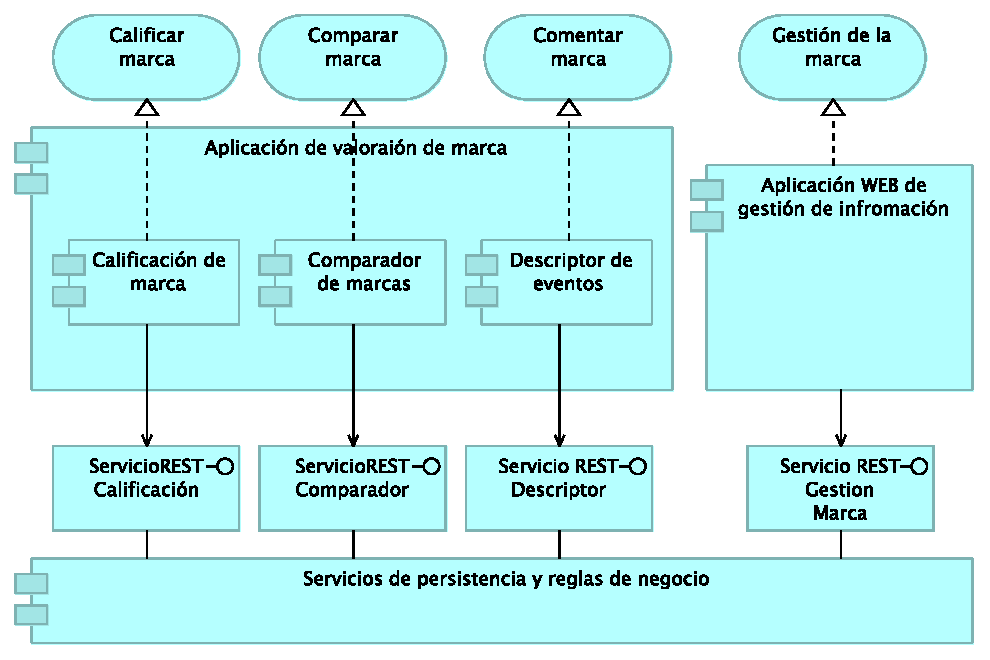
\includegraphics[scale=0.7]{Mestructuraaplicacion}
\caption{Punto de vista de Estrutura de aplicación.}
\label{Mestructuraaplicacion}
\end{figure}


\section{Uso de aplicación}

\marginpar{
    \begin{figure}[H]
        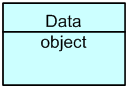
\includegraphics[scale=0.8]{IData_object}
    \end{figure} 
    \footnotesize 
    \textbf{Objeto de datos}. Un elemento pasivo que permite un proceso automatizado.
}

El punto de vista de uso de la aplicación se describe cómo se utilizan las aplicaciones para soportar uno o más procesos de negocio, y la forma en que son utilizados por otras aplicaciones. Puede ser utilizado en el diseño de una aplicación mediante la identificación de los servicios que necesitan los procesos de negocio y otras aplicaciones, o en el diseño de procesos de negocio mediante la descripción de los servicios que están disponibles. Por otra parte, ya que identifica las dependencias de los procesos de negocio en las aplicaciones, puede ser útil a los gestores operativos responsables de estos procesos.

\begin{figure}[H]
\centering
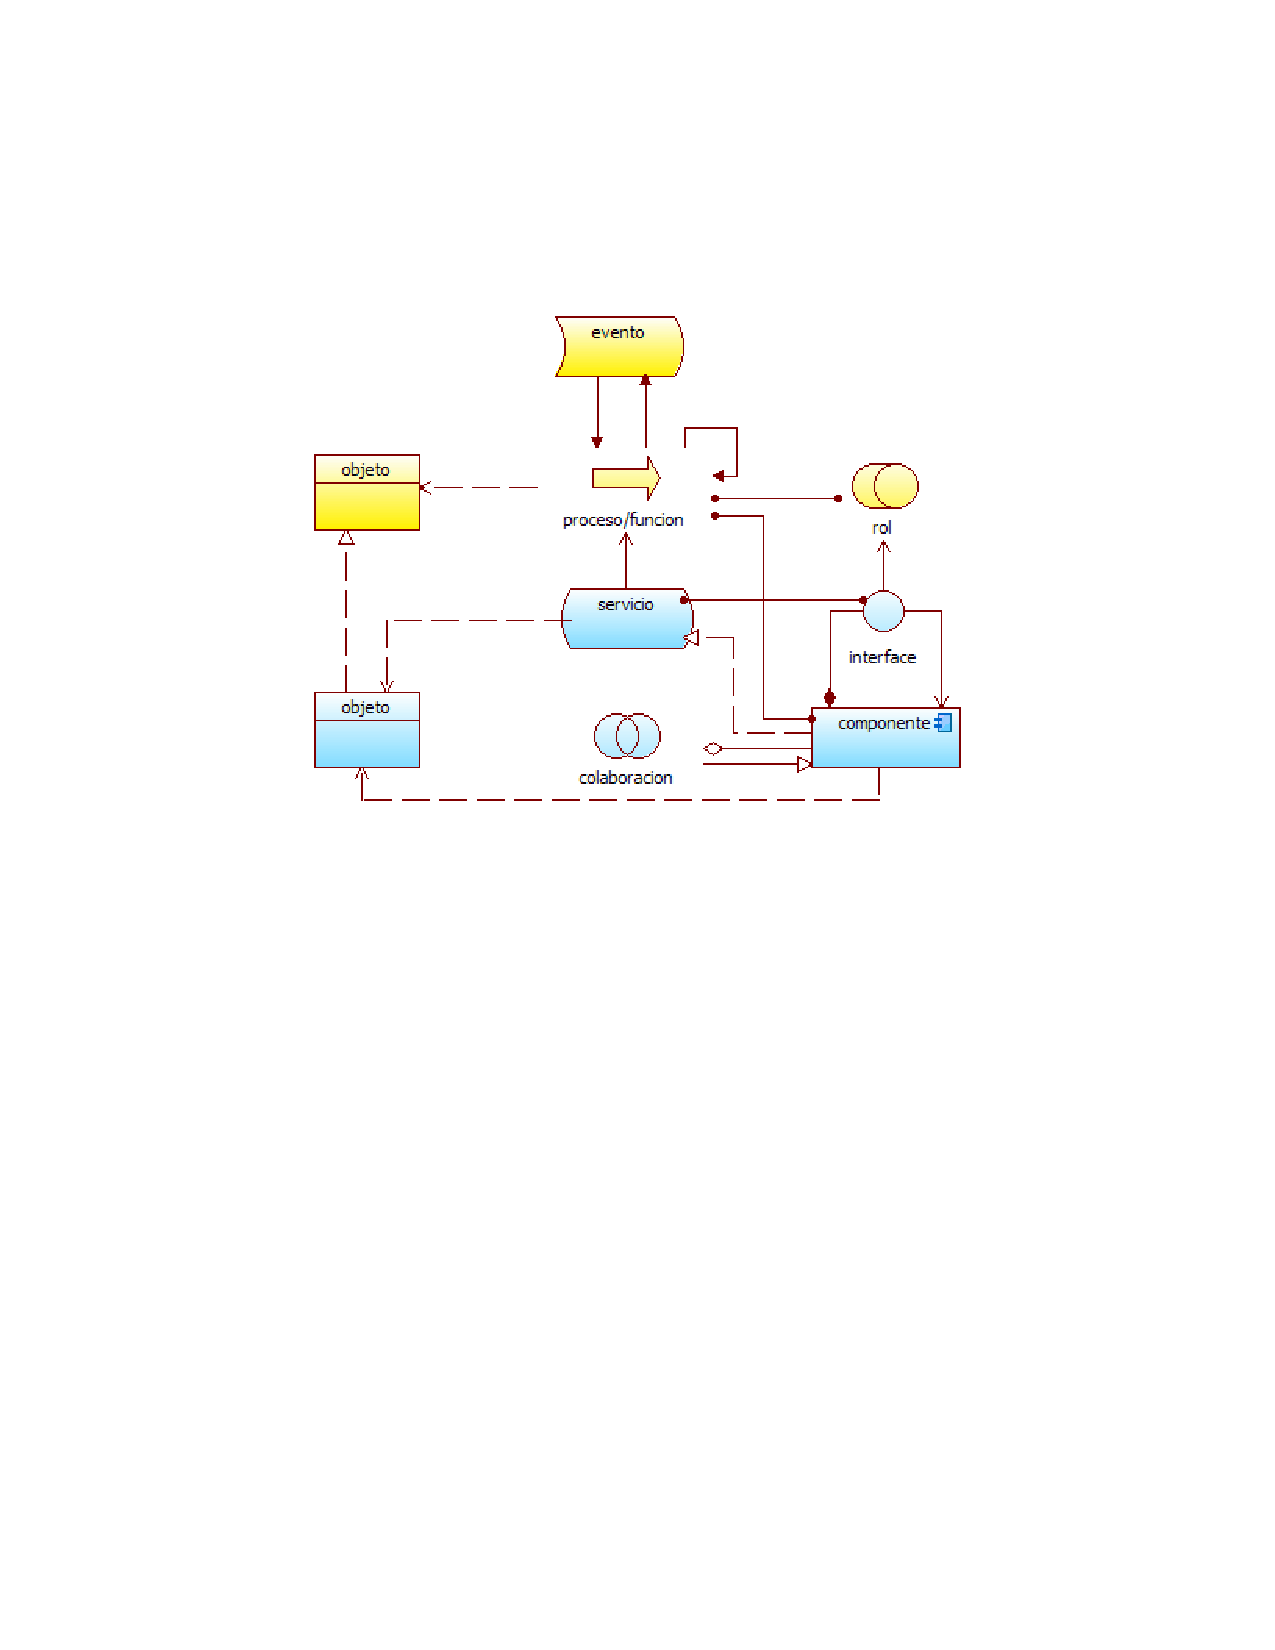
\includegraphics{uso_de_aplicacion}
\caption{Metamodelo del punto de vista de uso de aplicación.}
\end{figure}

Los procesos más importantes de la aplicación son realizados por unos componentes clave: la calificación de marca, la comparación entre marcas y la descripción de eventos entre marcas.

\begin{figure}[H]
\centering
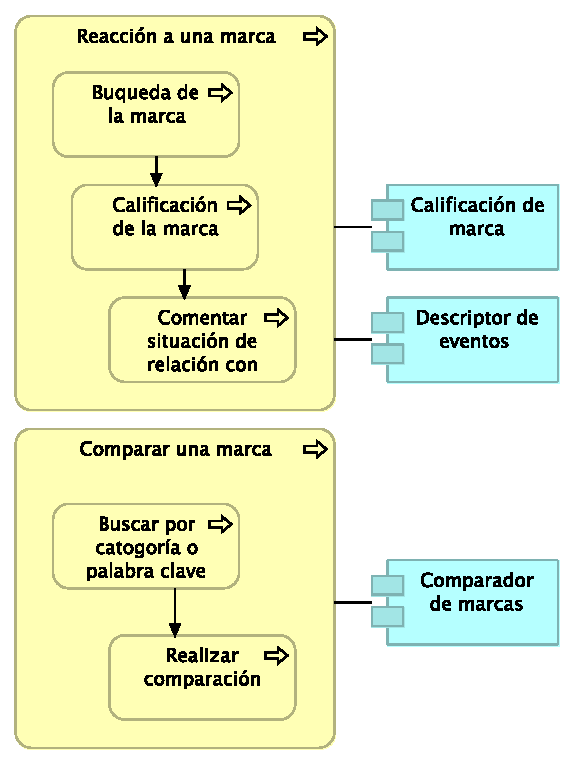
\includegraphics{Musoaplicacion}
\caption{Punto de vista de uso de aplicación.}
\end{figure}


